\chapter{Desenvolvimento}\label{chap:desenvolvimento}

O desenvolvimento do EIGAM conciliou modularidade, segurança, escalabilidade e capacidade de evolução. A solução foi construída como uma arquitetura de microsserviços orientada a eventos, na qual um barramento compatível com o \textit{Apache Kafka} conecta os serviços de forma assíncrona. Essa abordagem reduziu o acoplamento entre os componentes, distribuiu as responsabilidades de domínio e permitiu processar tarefas de forma independente, favorecendo a resiliência a picos de carga e a escalabilidade horizontal.

Segundo Newman (2022), microsserviços constituem uma abordagem na qual uma aplicação é organizada como um conjunto de serviços pequenos e independentes, responsáveis por capacidades específicas e passíveis de implantação e evolução separadas. No EIGAM, essa organização separou as responsabilidades de interação conversacional, identidade do titular, processamento financeiro, análise preditiva, notificações, geração de imagens, envio de mensagens, cobrança e auditoria. A modelagem do TCC~1 previa sete serviços; ao final do desenvolvimento, o sistema contava com treze componentes implantáveis, além de uma biblioteca compartilhada de contratos e de um \textit{design system} para as interfaces \textit{web}.

A arquitetura foi mantida desacoplada das plataformas de mensageria. O \textit{WhatsApp}, acessado pela \textit{Meta Cloud API}, permaneceu como canal principal, mas as regras de negócio não dependem dos formatos e recursos desse provedor. Uma camada de adaptadores converte as mensagens recebidas em representações internas padronizadas e, no sentido inverso, adapta as respostas às capacidades de cada canal. Essa decisão foi validada na prática: o \textit{Telegram} e a conversa dentro do painel \textit{web} do titular foram incorporados sem alterações nos serviços de domínio.

A camada de inteligência artificial seguiu a mesma premissa de separação de responsabilidades. O modelo de linguagem não é tratado como fonte de verdade dos dados financeiros, mas como recurso para ler a frase do usuário e redigir a resposta. Cálculos financeiros, validações de autorização, mascaramento de valores, comandos relacionados à LGPD e as análises preditivas permaneceram sob responsabilidade de mecanismos determinísticos ou estatísticos, executados pelos serviços que detêm os dados.

O processo de desenvolvimento seguiu práticas ágeis, com o \textit{backlog} organizado em \textit{sprints} temáticas, e utilizou testes automatizados desde o primeiro serviço. Além dos testes unitários e de integração, foram construídos conjuntos de referência rotulados (\textit{golden sets}) para medir a camada conversacional, testes de contrato entre os serviços implementados em linguagens diferentes, baterias com o modelo de linguagem real, um teste de carga no servidor de produção e um teste retrospectivo (\textit{backtest}) para a projeção de gastos. As decisões difíceis de reverter foram registradas em 37 \textit{Architecture Decision Records} (ADRs), documentos curtos que registram o contexto, a decisão tomada, as alternativas descartadas e o que mudaria a conclusão (Nygard, 2011).

\section{Arquitetura implementada}

O Quadro~\ref{frame:servicos} apresenta os componentes implantados e suas responsabilidades. Cada serviço é dono dos próprios dados e expõe a outros serviços apenas rotas internas ou eventos; nenhum serviço lê diretamente a tabela de outro.

{\small
\begin{longtable}{|L{3.4cm}|L{1.9cm}|L{9.2cm}|}
\caption{Componentes implementados} \label{frame:servicos} \\
\continuesmark
\hline
\textbf{Componente} & \textbf{Linguagem} & \textbf{Responsabilidade} \\ \hline
\endfirsthead
\hline
\textbf{Componente} & \textbf{Linguagem} & \textbf{Responsabilidade} \\ \hline
\endhead
\endfoot
\sourcerow{3} \\
\endlastfoot

\textit{API Gateway} & TypeScript & Recebe os \textit{webhooks} da Meta, do \textit{Telegram}, da Pluggy e do Stripe, valida a origem (HMAC ou segredo compartilhado), registra a mensagem de forma durável no barramento e responde imediatamente. Também serve os formulários dos Mini Apps do \textit{Telegram} e o \textit{endpoint} cifrado dos \textit{WhatsApp Flows}. \\ \hline
\textit{Identity Service} & TypeScript & Dono do titular: cadastro, identidades de canal, PIN, token de privilégio, sessões do painel e orquestração dos pedidos de exportação e exclusão de dados. \\ \hline
\textit{Chat Service} & TypeScript & Núcleo da conversa: aplica as regras determinísticas (LGPD, cadastro, PIN, bancos, metas), valida e executa o plano produzido pelo \textit{AI Service}, consulta o \textit{Finance Service}, aplica o mascaramento e guarda o histórico cifrado. \\ \hline
\textit{AI Service} & Python & Planejador que lê a frase do titular, redação da resposta, \textit{guardrails} de saída, base de conhecimento sobre o produto e transcrição de notas de voz. \\ \hline
\textit{Finance Service} & TypeScript & Sincronização com a Pluggy, categorização, pareamento de lançamentos, consultas financeiras, metas, detecção de sinais financeiros e cálculo dos resumos periódicos. \\ \hline
\textit{Analytics Service} & Python & Projeção de gastos até o fim do mês, com seleção de método por teste retrospectivo e abstenção quando a precisão não é suficiente. \\ \hline
\textit{Notification Service} & TypeScript & Política de avisos (preferências, janela de envio, agrupamento e deduplicação), agendamento dos resumos semanais e mensais e campanhas da equipe de operação. \\ \hline
\textit{Render Service} & TypeScript & Gera as imagens enviadas na conversa (gráficos, comprovantes e cartões) e os relatórios em PDF, desenhados em HTML e SVG e fotografados pelo Chromium. \\ \hline
\textit{Outbound Worker} & TypeScript & Envia as mensagens pelo adaptador de cada canal (\textit{WhatsApp}, \textit{Telegram} e \textit{web}), com limite de taxa, novas tentativas, \textit{circuit breaker} por canal e fila de mensagens com falha. \\ \hline
\textit{Billing Service} & TypeScript & Assinaturas no Stripe, controle de acesso por plano e cálculo do custo variável de cada titular a partir das unidades consumidas. \\ \hline
\textit{Audit Service} & TypeScript & Consome o tópico de auditoria e grava o registro imutável, encadeado por \textit{hash}. \\ \hline
Painel do titular & TypeScript (React) & Interface \textit{web} em \texttt{app.eigam.com.br} para consulta longa e gestão: mês, transações, cartões, recorrências, metas, investimentos, bancos, assinatura, privacidade e conversa. \\ \hline
Painel de operação & TypeScript (React) & Interface da equipe, atrás do Cloudflare Access: titulares, custos, campanhas, parâmetros de operação, auditoria, pedidos da LGPD e um laboratório para testar respostas. \\ \hline
\end{longtable}
}

A comunicação assíncrona utiliza o Redpanda, um \textit{broker} compatível com a API do Kafka. Os tópicos são particionados pelo identificador do titular (\texttt{user\_id}), o que garante a ordem das mensagens de cada pessoa sem serializar o sistema inteiro. Campos pessoais e financeiros são cifrados antes da produção do evento, de modo que o \textit{broker} armazena apenas texto cifrado. A Figura~\ref{fig:sequencia_turno} apresenta o caminho de uma mensagem do titular até a resposta.

\begin{figure}[htbp]
    \centering
    \caption{Processamento de uma mensagem do titular}
    \label{fig:sequencia_turno}
    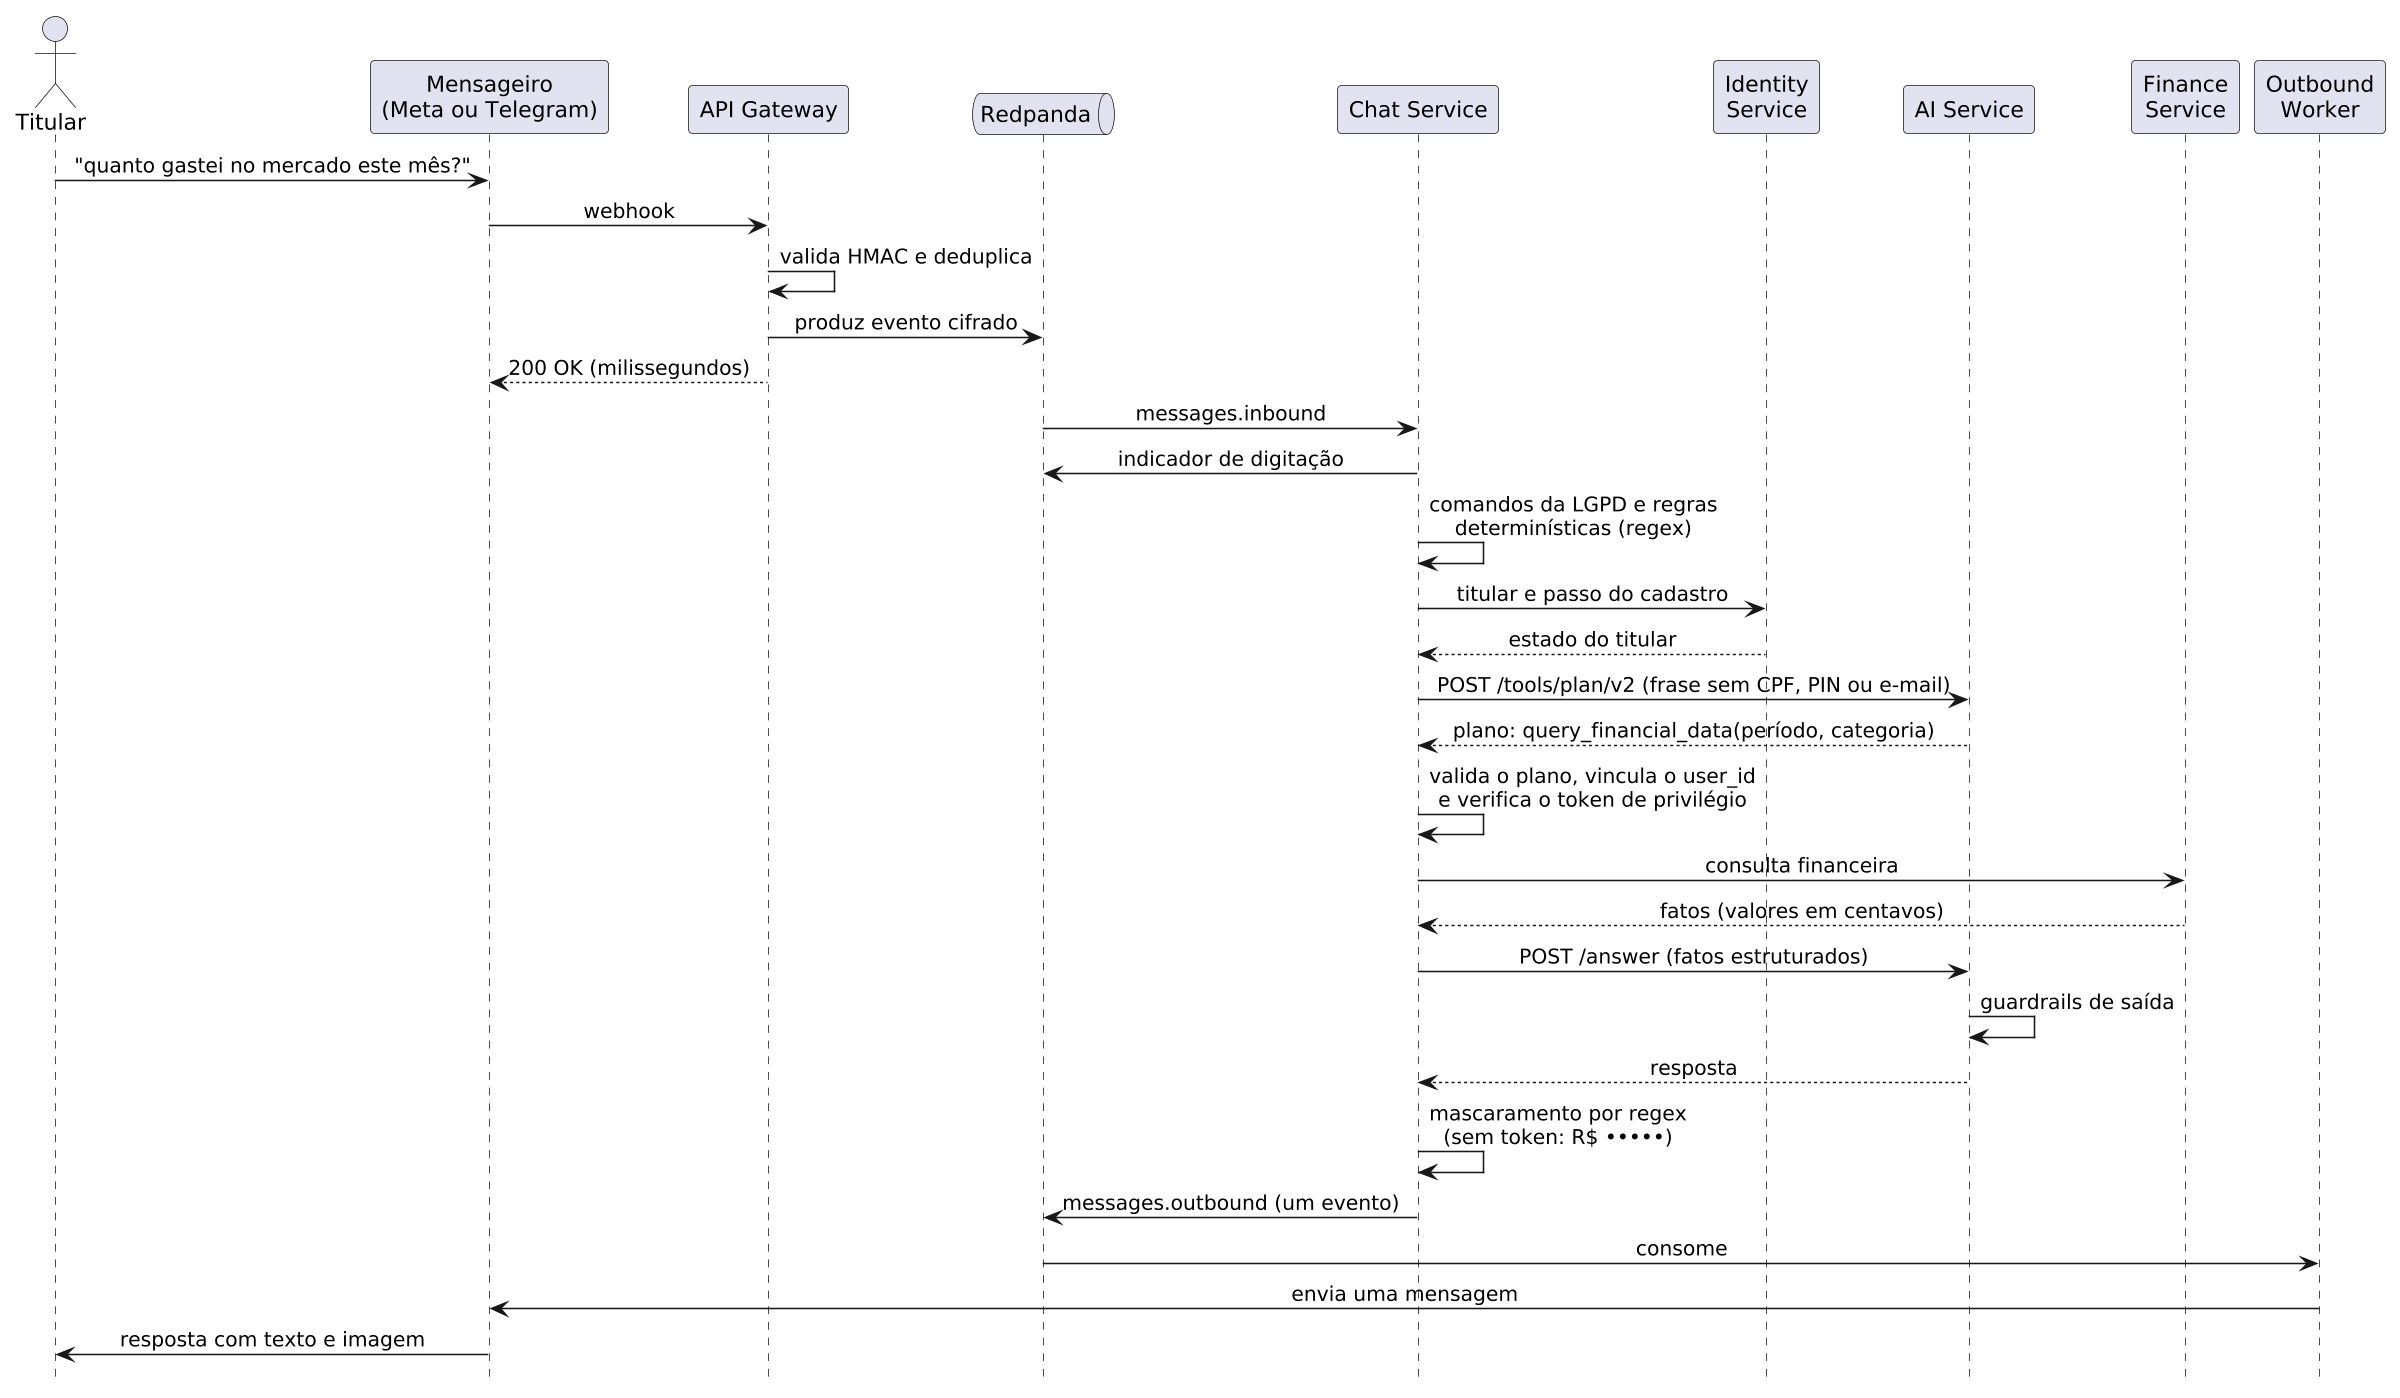
\includegraphics[width=\textwidth]{images/sequencia/processamento_mensagem.png}
    \authorssource
\end{figure}

O \textit{API Gateway} valida a assinatura do \textit{webhook}, marca a mensagem para deduplicação, publica o evento cifrado e responde ao provedor em poucos milissegundos, sem aguardar banco de dados ou modelo de linguagem. Um consumidor do próprio \textit{gateway} resolve o titular e publica o evento de domínio. O \textit{Chat Service} consome a mensagem, verifica primeiro os comandos da LGPD por expressões regulares e, em seguida, as regras determinísticas de cadastro, PIN, bancos, metas e recorrências. Apenas quando nenhuma regra decide o turno, a frase segue para o planejador do \textit{AI Service}, que escolhe quais consultas financeiras são necessárias. O \textit{Chat Service} valida esse plano, executa as consultas no \textit{Finance Service}, faz as contas em centavos e solicita a redação ao \textit{AI Service}. Por fim, aplica o mascaramento conforme o token de privilégio e publica um único evento de saída, enviado pelo \textit{Outbound Worker}.

\section{Tecnologias utilizadas}

O Quadro~\ref{frame:tecnologias} apresenta as tecnologias efetivamente empregadas no desenvolvimento. Em relação ao planejamento do TCC~1, a principal mudança foi a infraestrutura: em vez de serviços gerenciados em planos gratuitos, adotou-se um servidor na Hetzner Cloud descrito integralmente em Terraform, com broker, bancos e observabilidade executados em contêineres. A geração de gráficos também mudou: o Chart.js deu lugar a páginas HTML e SVG fotografadas pelo Chromium, que permitiram imagens com a identidade visual do produto e com logotipos de bancos e aplicativos.

{\small
\begin{longtable}{|L{3.2cm}|L{2.8cm}|L{6.7cm}|L{1.5cm}|}
\caption{Tecnologias utilizadas} \label{frame:tecnologias} \\
\continuesmark
\hline
\textbf{Nome} & \textbf{Fornecedor} & \textbf{Descrição} & \textbf{Versão} \\ \hline
\endfirsthead
\hline
\textbf{Nome} & \textbf{Fornecedor} & \textbf{Descrição} & \textbf{Versão} \\ \hline
\endhead
\endfoot
\sourcerow{4} \\
\endlastfoot

Git & Open Source & Controle de versão dos dezessete repositórios do projeto, agregados por submódulos em um monorrepositório. & 2.x \\ \hline
GitHub & Microsoft & Hospedagem dos repositórios privados, integração contínua com GitHub Actions, registro de imagens (GHCR) e publicação dos pacotes compartilhados. & -- \\ \hline
Node.js & OpenJS Foundation & Ambiente de execução dos serviços escritos em TypeScript. & 20 LTS \\ \hline
TypeScript & Microsoft & Tipagem estática em todos os serviços Node.js e nos painéis \textit{web}. & 5.6 \\ \hline
Fastify & Open Source & \textit{Framework} HTTP do \textit{gateway}, das rotas internas dos serviços e da API dos painéis. & 5.1 \\ \hline
Python & Python Software Foundation & Linguagem do \textit{AI Service} e do \textit{Analytics Service}, por causa do ecossistema de modelos de linguagem e de estatística. & 3.12 \\ \hline
FastAPI e Pydantic & Open Source & \textit{Framework} HTTP e validação de dados dos serviços Python. & 0.115 / 2.9 \\ \hline
Redpanda & Redpanda Data & \textit{Broker} compatível com a API do Kafka, executado em contêiner com 1 GB de memória. & 24.2 \\ \hline
KafkaJS e aiokafka & Open Source & Clientes do \textit{broker} nos serviços TypeScript e Python. & 2.2 / 0.12 \\ \hline
Redis & Redis Ltd. & Sessões, token de privilégio, estado de conversa, cache, limitação de taxa e filas. & 7.4 \\ \hline
BullMQ & Open Source & Filas e tarefas agendadas sobre o Redis: sincronização, resumos e varreduras. & 5.34 \\ \hline
PostgreSQL & Open Source & Banco relacional: titulares, consentimentos, metas, assinaturas, custos, auditoria e operação. & 16 \\ \hline
pgcrypto e pgvector & Open Source & Cifragem de colunas no banco e suporte a vetores, ambos na imagem \texttt{pgvector/pgvector:pg16}. & -- \\ \hline
MongoDB Atlas & MongoDB, Inc. & Banco documental gerenciado para transações, saldos, faturas, investimentos, empréstimos, histórico de conversa e previsões. & -- \\ \hline
Drizzle ORM e Mongoose & Open Source & Acesso tipado ao PostgreSQL e ao MongoDB. O esquema relacional é mantido em 51 migrações SQL versionadas. & 0.36 / 8 \\ \hline
Zod & Open Source & Validação dos contratos de eventos, rotas e configurações, compartilhada entre os serviços pelo pacote \texttt{@eigam-corp/shared}. & 3.23 \\ \hline
OpenAI API & OpenAI & Modelo de linguagem do planejador e da redação das respostas (\texttt{gpt-5.6-luna}) e transcrição de notas de voz. & -- \\ \hline
TypeSafe (JEV) & TypeSafe & Modelo de juízo tipado usado pelos \textit{guardrails} de conselho regulado e de \textit{prompt injection}. & -- \\ \hline
Meta Cloud API & Meta & Canal \textit{WhatsApp}, encapsulado pelo adaptador de canal, incluindo mensagens interativas, \textit{templates} e \textit{WhatsApp Flows}. & v21+ \\ \hline
Telegram Bot API & Telegram & Segundo canal de mensageria, com teclados interativos e Mini Apps para os formulários. & -- \\ \hline
Pluggy & Pluggy & Agregador de dados de \textit{Open Finance}: conexão com as instituições, transações, saldos, faturas, investimentos e empréstimos. & v1 \\ \hline
Stripe & Stripe & Assinaturas recorrentes do plano Pro, \textit{checkout} e portal do cliente. & -- \\ \hline
React, Vite e Tailwind CSS & Open Source & Interfaces dos dois painéis \textit{web} e do \textit{design system} \texttt{@eigam-corp/ui}. & 18.3 / 5.4 / 4 \\ \hline
Puppeteer e Chromium & Google & Fotografia das páginas HTML e SVG que geram as imagens e os PDFs enviados ao titular. & 24 \\ \hline
Docker e Docker Compose & Docker, Inc. & Conteinerização de todos os serviços e da infraestrutura de apoio. & 27+ \\ \hline
Terraform & HashiCorp & Infraestrutura como código: servidor, firewall, rede privada, volume cifrado, DNS e túnel da Cloudflare. & 1.x \\ \hline
Hetzner Cloud & Hetzner & Servidor CX33 (4 vCPU, 8 GB de RAM) em Falkenstein, na Alemanha. & -- \\ \hline
Cloudflare & Cloudflare & \textit{Proxy} na borda, DNS, túnel para os painéis e autenticação da equipe com o Cloudflare Access. & -- \\ \hline
Nginx e Let's Encrypt & Open Source / ISRG & \textit{Reverse proxy} com terminação TLS e certificados renovados automaticamente. & 1.27 \\ \hline
SOPS e age & Open Source & Segredos versionados cifrados no repositório e decifrados somente no momento da implantação. & -- \\ \hline
Prometheus, Loki, Tempo e Grafana & Grafana Labs / CNCF & Métricas, \textit{logs}, rastreamento distribuído, painéis e alertas, todos executados no próprio servidor. & 3.6 / 3.5 / 2.9 / 12.2 \\ \hline
Vitest e Pytest & Open Source & Testes unitários, de integração e de cobertura nos serviços TypeScript e Python. & 2.1 / 8 \\ \hline
Claude Code & Anthropic & Assistente de programação utilizado pela equipe, com o \textit{backlog} e a referência de arquitetura versionados como habilidades do próprio repositório. & -- \\ \hline

\end{longtable}
}

\subsection{Integração Multicanal}

A comunicação com as plataformas de mensageria foi implementada por adaptadores que isolam as particularidades de cada provedor. A identidade do usuário deixou de ser o número de telefone e passou a ser um identificador interno (\texttt{user\_id}) com qualquer número de identidades de canal: o telefone no \textit{WhatsApp}, o identificador de conversa no \textit{Telegram} e o próprio \texttt{user\_id} no painel \textit{web}. Assim, uma mesma pessoa pode conversar pelos três canais com o mesmo cadastro, o mesmo PIN e os mesmos dados.

O núcleo trabalha com intenções de resposta (texto, imagem, documento, formulário e mensagem interativa), e cada adaptador declara as capacidades do seu canal. Um formulário, por exemplo, vira \textit{WhatsApp Flow} no \textit{WhatsApp}, Mini App no \textit{Telegram} e conversa guiada onde não houver recurso equivalente. Os onze formulários do produto, como cadastro, conexão de banco, metas, preferências e direitos do titular, são definidos uma única vez e traduzidos para cada canal. Os \textit{WhatsApp Flows} trocam dados com o \textit{gateway} por um \textit{endpoint} cifrado, conforme a especificação da Meta.

Uma restrição comercial também moldou essa camada. Durante o desenvolvimento, a Meta passou a cobrar mensagens de serviço que antes eram gratuitas. Por isso, cada gatilho, seja mensagem do titular, alerta ou resumo, passou a produzir uma única mensagem: o texto que acompanha uma imagem vai na legenda, o que acompanha um botão vai no corpo da mensagem interativa, e avisos de progresso viraram indicador de digitação, que não é cobrado.

\subsection{Camada de Inteligência Artificial}

A leitura da frase do titular é feita por um planejador baseado em chamada de funções (\textit{function calling}). O modelo de linguagem não responde ao usuário nessa etapa: ele apenas escolhe, entre sete funções de um contrato versionado, quais consultas são necessárias e com quais argumentos (período, instituição, categoria, estabelecimento, forma de pagamento e agrupamento). O \textit{Chat Service} revalida os argumentos com os mesmos esquemas usados pelos demais serviços, vincula o identificador do titular, que nunca é argumento do modelo, e executa as consultas. O planejador tem até 4,5 segundos, com uma segunda tentativa, e o \textit{Chat Service} desiste em 4,7 segundos; nesse caso, o titular recebe uma recusa sem número, em vez de um valor possivelmente errado.

Na resposta, os fatos consultados são enviados ao modelo como dados estruturados, única fonte autorizada de valores. Para as consultas mais comuns, o servidor monta as linhas com os números exatos e o modelo escreve apenas a abertura, a leitura e a oferta do próximo passo, conferidas pelo servidor. Perguntas sobre o próprio produto, como planos, segurança e funcionamento do \textit{Open Finance}, são respondidas a partir de uma base de conhecimento escrita pela equipe e recuperada por palavras-chave.

Os \textit{guardrails} de saída verificam conselho de investimento ou tributário, pedido de credencial, vazamento de instruções internas, \textit{prompt injection}, contatos não informados pelo titular, comprimento da resposta e ofertas não autorizadas. O conselho regulado e a injeção são avaliados por expressões regulares e, de forma complementar, por um modelo de juízo tipado; a decisão final é a união dos dois. O mascaramento de valores ocorre depois de tudo isso, no publicador do \textit{Chat Service}, por expressão regular.

Notas de voz são transcritas pelo \textit{AI Service} e seguem o mesmo caminho do texto, inclusive a verificação dos comandos da LGPD. O áudio não é armazenado, e a transcrição é guardada cifrada no histórico.

\subsection{Análise Preditiva e Sinais Financeiros}

A categoria de cada transação passou a ser a do conector de \textit{Open Finance}, organizada em uma taxonomia de dois níveis com 95 categorias em 17 grupos, decidida uma única vez na sincronização e sem uso de modelo de linguagem. O \textit{Finance Service} também pareia as duas pernas de um mesmo evento, como o pagamento de fatura e a compra que ele quita, ou a compra e o seu estorno. Sem esse pareamento, o mesmo gasto seria contado duas vezes.

A projeção de gastos do mês é calculada pelo \textit{Analytics Service} a partir da série diária fornecida pelo \textit{Finance Service}. Três métodos candidatos, o ritmo atual do mês, a mediana histórica e uma média móvel exponencialmente ponderada (EWMA), são avaliados por teste retrospectivo sobre os meses anteriores. Um critério de aprovação exige erro percentual absoluto ponderado (WAPE) de até 20\%, viés absoluto de até 5\%, cobertura do intervalo de 80\% entre 70\% e 90\% e ganho mínimo de 10\% sobre o método de referência. Quando nenhum candidato atende ao critério, o sistema se abstém de apresentar um número e informa que ainda não há dados suficientes para uma projeção confiável.

Os sinais financeiros nascem no \textit{Finance Service}, onde estão os dados, e seguem cifrados para o \textit{Notification Service}, que decide se e quando avisar. Foram implementados seis sinais: limite de gasto atingido em 80\% e em 100\%, risco de ultrapassar o limite até o fim do período, possível cobrança duplicada, transação atípica e aumento de gasto em uma categoria. A transação atípica utiliza um escore-z robusto sobre o logaritmo do valor, calculado com a mediana e o desvio absoluto mediano do histórico da mesma categoria, com limiar de 3,5 e exigência mínima de dez transações e noventa dias de histórico. O titular escolhe quais famílias de aviso deseja receber e em qual janela de horário.

Os resumos semanal e mensal são gerados sob adesão explícita do titular. O \textit{Notification Service} agenda os pedidos, o \textit{Finance Service} calcula os números e o \textit{Render Service} produz um relatório em PDF. O aviso enviado ao titular não contém valores, e a abertura do relatório exige o token de privilégio, como qualquer outro valor.

\subsection{Segurança e Privacidade}

Os campos sensíveis são cifrados antes de sair do processo que os produziu: com \texttt{pgcrypto} no PostgreSQL, com AES-256-GCM na aplicação para o MongoDB e o Redis, e no próprio conteúdo dos eventos do \textit{broker}. A chave de cada titular é derivada por HKDF a partir de uma chave mestra e do \texttt{user\_id}. Colunas que precisam de busca possuem uma coluna irmã com HMAC-SHA256, e o volume do PostgreSQL é cifrado com LUKS. Como o \textit{Analytics Service}, escrito em Python, decifra os mesmos campos que os serviços TypeScript, ambos são testados contra os mesmos vetores fixos de criptografia.

O PIN de seis dígitos é armazenado com \textit{bcrypt} e, após cinco tentativas incorretas, o acesso é bloqueado por 30 minutos. O PIN correto emite um token de privilégio com validade de 8 horas, ajustável entre 1 e 24 horas pelo painel de operação. Sem esse token, os valores aparecem como \texttt{R\$ •••••} na conversa, nas imagens e no painel do titular. O registro de auditoria é somente de inserção, encadeado por \textit{hash} SHA-256 e guarda referências em vez de dados pessoais, para poder ser mantido por cinco anos mesmo após a exclusão da conta.

Os direitos do titular são exercidos por mensagem em qualquer canal. O \textit{Chat Service} reconhece o comando, solicita o PIN e a confirmação e registra o pedido; o \textit{Identity Service} executa a exportação e a exclusão, coordenando os serviços donos de cada dado. A exportação gera um arquivo JSON entregue como documento no próprio canal do pedido, sem link nem armazenamento intermediário.

\subsection{Painéis \textit{Web}}

Durante o desenvolvimento, dois painéis \textit{web} foram incorporados ao escopo. O painel de operação atende à equipe: mostra onde os titulares param no cadastro, o custo por conversa e por titular, a saúde das conexões bancárias, as campanhas, os parâmetros de operação, a auditoria e os pedidos da LGPD. O acesso passa pelo Cloudflare Access, e cada operador recebe papéis específicos, como leitor de conversas ou editor de parâmetros.

O painel do titular estende a conversa, sem substituí-la. O acesso ocorre pelo número do \textit{WhatsApp}, que recebe um código de seis dígitos, ou por um link de uso único enviado na conversa. O painel não tem banco de dados próprio: cada requisição recebe do \textit{Identity Service} uma credencial de cinco minutos, e os serviços de dados identificam o titular por essa credencial. Os direitos da LGPD continuam sendo exercidos pela conversa: os botões da tela abrem o mensageiro com o comando já escrito. Desde 30/10/2026, o painel também possui uma conversa com o EIGAM, implementada como um terceiro canal (\textit{web}), atendido por um novo adaptador no \textit{Outbound Worker}.

\subsection{Infraestrutura e Implantação}

Toda a infraestrutura foi descrita em Terraform: um servidor CX33 na Hetzner Cloud, um volume de 40 GB cifrado com LUKS para o PostgreSQL, rede privada, \textit{firewall} que aceita tráfego HTTP apenas das faixas da Cloudflare, registros DNS e o túnel dos painéis. O servidor fica em Falkenstein, na Alemanha, e o MongoDB Atlas, em Frankfurt; todos os dados pessoais permanecem na União Europeia.

Cada serviço publica uma imagem no registro do GitHub ao entrar na \textit{branch} principal, identificada pelo \textit{hash} do \textit{commit}. A versão que vai ao ar é declarada em um único arquivo do repositório de infraestrutura; alterar esse arquivo dispara a implantação, que decifra os segredos, aplica as migrações, cria os tópicos, sobe os contêineres, confere se as imagens em execução correspondem às declaradas e aguarda os serviços ficarem saudáveis. Voltar uma versão é editar uma linha. A observabilidade, com Prometheus, Loki, Tempo, Grafana e Alertmanager, roda no próprio servidor, e o Grafana não fica exposto à internet.

\section{Metodologias e padrões de software}

Os padrões e práticas de engenharia de software são fundamentais para garantir a coerência, a manutenibilidade e a capacidade de evolução de sistemas distribuídos. Segundo Bass, Clements e Kazman (2022), decisões arquiteturais influenciam diretamente atributos como desempenho, segurança, disponibilidade e modificabilidade e, portanto, devem ser explicitamente definidas e documentadas. O Quadro~\ref{frame:padroes} apresenta as abordagens adotadas no EIGAM.

{\small
\begin{longtable}{|L{4.5cm}|L{10cm}|}
\caption{Metodologias e padrões adotados} \label{frame:padroes} \\
\continuesmark
\hline
\textbf{Nome} & \textbf{Descrição} \\ \hline
\endfirsthead
\hline
\textbf{Nome} & \textbf{Descrição} \\ \hline
\endhead
\endfoot
\sourcerow{2} \\
\endlastfoot

Metodologia Scrum & O desenvolvimento foi organizado em 14 \textit{sprints} temáticas, ordenadas por dependência técnica, com \textit{backlog} de 223 cartões e critérios de aceitação verificáveis em cada um. \\ \hline
Arquitetura de microsserviços orientada a eventos & Serviços separados por responsabilidade de domínio, cada um dono dos próprios dados, comunicando-se por eventos no Redpanda e por rotas HTTP internas quando há necessidade de resposta imediata. \\ \hline
Separação em camadas & Cada serviço separa rotas e validação de entrada, regras de aplicação e acesso a dados, de modo que a regra de negócio não dependa do formato HTTP nem do banco. \\ \hline
Adapter & Utilizado nos canais de mensageria e nos demais fornecedores. O nome do fornecedor aparece apenas no adaptador: eventos, tabelas e serviços de domínio usam vocabulário próprio do EIGAM. \\ \hline
Strategy & Utilizado na projeção de gastos, em que métodos candidatos com a mesma interface são escolhidos pelo resultado do teste retrospectivo. \\ \hline
\textit{Function calling} e recuperação de contexto & O modelo de linguagem escolhe funções de um contrato tipado em vez de produzir texto livre; os fatos chegam ao prompt por consultas estruturadas, e o conhecimento sobre o produto, por recuperação por palavras-chave. \\ \hline
\textit{Circuit Breaker}, \textit{Retry} e fila de falhas & Integrações externas com novas tentativas e \textit{backoff} exponencial, interrupção temporária por canal quando a taxa de erro passa de 50\% e fila de mensagens com falha para reprocessamento. \\ \hline
Idempotência e deduplicação & \textit{Webhooks}, eventos de cobrança e envios de aviso são deduplicados, de forma que um reenvio do provedor não gere cobrança ou mensagem repetida. \\ \hline
Infraestrutura como código & Todo recurso de infraestrutura existe apenas no Terraform, e toda versão em produção é declarada em arquivo versionado. \\ \hline
Registro de decisões de arquitetura (ADR) & As 37 decisões difíceis de reverter foram documentadas com contexto, decisão, alternativas descartadas e critérios que mudariam a conclusão. \\ \hline
TDD (\textit{Test-Driven Development}) & Testes automatizados orientaram a implementação das regras determinísticas, como mascaramento, comandos da LGPD, leitura de metas e cálculos financeiros. \\ \hline
\textit{Conventional Commits} & Mensagens de \textit{commit} padronizadas por tipo (\texttt{feat}, \texttt{fix}, \texttt{docs}, \texttt{refactor}), o que facilitou a leitura do histórico de mais de 2.500 \textit{commits}. \\ \hline

\end{longtable}
}

\section{Metodologia de testes de software}

A estratégia de testes do EIGAM foi composta por diferentes níveis, adequados à natureza distribuída da aplicação. Segundo Richardson (2019), em arquiteturas de microsserviços, a validação isolada dos serviços deve ser complementada por testes das integrações, pois falhas podem ocorrer não apenas na lógica interna, mas também nos contratos entre componentes independentes.

Os testes unitários e de integração foram escritos com Vitest nos serviços TypeScript e com Pytest nos serviços Python. A integração contínua executa, a cada alteração, a análise estática, a verificação de tipos, os testes com medição de cobertura e o \textit{build}; cada pacote TypeScript exige cobertura mínima de 70\% em linhas, funções, ramificações e instruções. Os contratos de eventos e de rotas são esquemas compartilhados pelo pacote \texttt{@eigam-corp/shared}, e a criptografia, implementada em duas linguagens, é verificada contra vetores fixos comuns.

A camada conversacional foi avaliada com \textit{golden sets}: conjuntos de frases e conversas rotuladas, versionados no repositório de documentação. Há conjuntos para mascaramento, comandos da LGPD, leitura de metas, ações sobre bancos, consultas financeiras, \textit{guardrails}, \textit{prompt injection}, cadastro, transcrição de áudio e perguntas difíceis. Os conjuntos que dependem apenas de regras determinísticas exigem 100\% de acerto. As instruções e as funções do planejador têm o \textit{hash} fixado em teste, de modo que qualquer mudança no prompt sem decisão registrada falha na integração contínua. Os conjuntos que dependem do modelo real foram executados em baterias pagas fora da integração contínua, e a qualidade das respostas abertas foi avaliada por um segundo modelo de linguagem atuando como juiz, com notas de 0 a 10.

O desempenho foi medido por um teste de carga no próprio servidor de produção, em rede isolada, com um modelo de linguagem simulado que reproduz planos e tempos reais gravados. A projeção de gastos foi avaliada por teste retrospectivo, comparando cada previsão com o valor que de fato ocorreu. Por fim, o painel de operação oferece um laboratório que executa o turno completo em produção, com a conta do próprio operador, mostrando o caminho da mensagem, as chamadas aos modelos e o custo de cada resposta. Os resultados dessas medições são apresentados no Capítulo~\ref{chap:resultados}.

\section{Métricas de qualidade}

Segundo Bass, Clements e Kazman (2022), atributos de qualidade são propriedades mensuráveis de um sistema que indicam quão bem ele satisfaz as necessidades de seus \textit{stakeholders}. Em sistemas distribuídos orientados a eventos, características como disponibilidade, desempenho, segurança, modificabilidade e observabilidade precisam ser consideradas desde a arquitetura. No EIGAM, também foi necessário avaliar atributos específicos da camada de inteligência artificial e da integração multicanal. O Quadro~\ref{frame:metricas} apresenta os objetivos de qualidade adotados, cujos resultados medidos são discutidos no Capítulo~\ref{chap:resultados}.

{\small
\begin{longtable}{|L{4cm}|L{10.5cm}|}
\caption{Métricas de qualidade} \label{frame:metricas} \\
\continuesmark
\hline
\textbf{Fator de Qualidade} & \textbf{Objetivo} \\ \hline
\endfirsthead
\hline
\textbf{Fator de Qualidade} & \textbf{Objetivo} \\ \hline
\endhead
\endfoot
\sourcerow{2} \\
\endlastfoot

Manutenibilidade &
\begin{minipage}[t]{\linewidth}
\begin{itemize}[noitemsep,topsep=2pt,leftmargin=*]
    \item Serviços com responsabilidades delimitadas e donos dos próprios dados.
    \item TypeScript com tipagem estrita e contratos validados por esquemas compartilhados.
    \item Cobertura mínima de 70\% exigida pela integração contínua em todos os pacotes TypeScript.
    \item Adaptadores de canal e de fornecedor isolados das regras de negócio.
\end{itemize}
\end{minipage} \\ \hline

Desempenho &
\begin{minipage}[t]{\linewidth}
\begin{itemize}[noitemsep,topsep=2pt,leftmargin=*]
    \item \textit{Webhooks} confirmados em milissegundos, com todo o processamento fora da requisição.
    \item Resposta conversacional em torno de 4 segundos, pois acima disso o usuário tende a concluir que o assistente travou.
    \item Planejador limitado a 4,5 segundos, com recusa sem número quando o prazo é excedido.
\end{itemize}
\end{minipage} \\ \hline

Disponibilidade e Resiliência &
\begin{minipage}[t]{\linewidth}
\begin{itemize}[noitemsep,topsep=2pt,leftmargin=*]
    \item \textit{Circuit breaker} por canal, novas tentativas com \textit{backoff} e fila de mensagens com falha.
    \item \textit{Webhook} registrado de forma durável antes da resposta ao provedor.
    \item \textit{Healthchecks} dos contêineres e verificação das versões em execução a cada implantação.
    \item Conversa e comandos da LGPD disponíveis mesmo com o \textit{Finance Service} ou o modelo de linguagem indisponíveis.
\end{itemize}
\end{minipage} \\ \hline

Segurança e Conformidade LGPD &
\begin{minipage}[t]{\linewidth}
\begin{itemize}[noitemsep,topsep=2pt,leftmargin=*]
    \item Campos sensíveis cifrados antes de sair do processo, em todos os bancos e no \textit{broker}.
    \item Token de privilégio de 8 horas, ajustável entre 1 e 24 horas.
    \item Mascaramento determinístico com 100\% de conformidade no \textit{golden set}.
    \item Reconhecimento dos comandos da LGPD com 100\% de revocação, sem depender do modelo.
    \item Auditoria somente de inserção, encadeada por \textit{hash} e retida por cinco anos.
\end{itemize}
\end{minipage} \\ \hline

Portabilidade e Interoperabilidade &
\begin{minipage}[t]{\linewidth}
\begin{itemize}[noitemsep,topsep=2pt,leftmargin=*]
    \item Serviços conteinerizados e configuração por variáveis de ambiente.
    \item Contratos internos padronizados para entrada e saída de mensagens, comprovados pelo funcionamento simultâneo de três canais.
\end{itemize}
\end{minipage} \\ \hline

Usabilidade &
\begin{minipage}[t]{\linewidth}
\begin{itemize}[noitemsep,topsep=2pt,leftmargin=*]
    \item Interação pelos mensageiros já presentes na rotina do usuário.
    \item Uma mensagem por interação, com imagem e texto juntos quando a resposta pede gráfico.
    \item Formulários nativos de cada canal para cadastro, conexão de banco, metas, preferências e direitos do titular.
\end{itemize}
\end{minipage} \\ \hline

Confiabilidade da Inteligência Artificial &
\begin{minipage}[t]{\linewidth}
\begin{itemize}[noitemsep,topsep=2pt,leftmargin=*]
    \item Valores apresentados apenas a partir de dados estruturados consultados no turno.
    \item Macro-F1 mínimo de 0,88 na classificação do motivo pelo planejador.
    \item 100\% de bloqueio e 100\% de preservação nos conjuntos de \textit{guardrails} e de \textit{prompt injection}.
    \item Projeção apresentada apenas quando aprovada no teste retrospectivo; caso contrário, abstenção declarada.
\end{itemize}
\end{minipage} \\ \hline

Observabilidade &
\begin{minipage}[t]{\linewidth}
\begin{itemize}[noitemsep,topsep=2pt,leftmargin=*]
    \item Métricas, \textit{logs} estruturados e rastreamento distribuído centralizados no Grafana.
    \item Alertas para latência do modelo, respostas de contingência frequentes, planejador sem plano, coleta bancária atrasada, fila de falhas com mensagens, disco, memória e disponibilidade dos serviços e do painel do titular.
    \item Custo de cada resposta registrado por turno e por titular.
\end{itemize}
\end{minipage} \\ \hline

\end{longtable}
}
